\documentclass[10pt]{article}
\usepackage{setspace}
\usepackage{amsmath,amsfonts,amsthm,amssymb}
\usepackage{color}
\usepackage{fancyhdr}
\usepackage{chngpage}
\usepackage{enumerate}
\usepackage{graphicx}
\usepackage{boxedminipage}

\title{Homework 10  in \LaTeX}
\author{Robert Brothers Mechanical Engineering Student @ UTSA}
\begin{document}
\doublespacing
\footnotesize
\maketitle
\date

\section{Interpreting Position & Velocity}
\subsection{(a) Starting position, velocity and acceleration}
\begin{equation}
\begin{align}
q_{0} &=
\begin{bmatrix}
10 \\
5  \\
\end{bmatrix}
\end{align}
\end{equation}

\subsection{(b) Find the Equation of Motion of the Particle}
\begin{equation}
\begin{align}
q_{f} &=
\begin{bmatrix}
21 \\
16 \\
\end{bmatrix}
\end{align}
\end{equation}

\section{Trajectory generation for given condition}
\subsection{(a) Minimal order}
For trajectory with initial conditions including position velocity and acceleration
we'd need a $4^{th}$ order polynomial.

\subsection{(b) joint position}
\begin{equation}
\begin{align}
\theta &= 
\end{align}
\end{equation}

\subsection{(c) plot $\theta\left(t\right)$, $\dot{\theta}\left(t\right)$ and $\ddot{\theta}\left(t\right)$}
Plots are in appendix

\section{Trajectory Generations with Points }
\subsection{(a) Find Cubic Polynomials that Fit Points}
\begin{equation}
q_{1}\left(t\right) &=
\begin{align}
 a_{0} + a_{1}t + a_{2}t^{2} + a_{3}t^{3}
\end{align}
\end{equation}

\subsection{(b) Plots of the position, velocity and acceleration}
plots are located in appendix


\section{Symbolic derivation of equations & simulations}
\subsection{(a) Expressions for center of mass}
\begin{equation}
r_{c1} &=
\begin{align}
\begin{bmatrix}
-n_{1} \\
0\\
0\\
1\\
\end{bmatrix}
\end{align}
\end{equation}

\begin{equation}
r_{c2} &=
\begin{align}
\begin{bmatrix}
-n_{2} \\
0\\
0\\
1\\
\end{bmatrix}
\end{align}
\end{equation}

\begin{equation}
r_{c3} &=
\begin{align}
\begin{bmatrix}
-n_{3} \\
0\\
0\\
1\\
\end{bmatrix}
\end{align}
\end{equation}

\subsection{(b) Location of Joints}
\begin{equation}
O_{0} &=  A_{0}^{0}O_{0}^{0}
\end{equation}

\begin{equation}
O_{1} &=  A_{1}^{0}O_{1}^{1}
\end{equation}

\begin{equation}
O_{2} &= A_{2}^{0}O_{2}^{2}
\end{equation}

\begin{equation}
O_{3} &= A_{3}^{0}O_{3}^{3}
\end{equation}

\subsection{(c) Translational Jacobians of Points}
\begin{equation}
J_{v1} &= 
\begin{bmatrix}
R_{0}^{0} \hat{k} \times \left(r_{c1} - O_{0}\right) & 0 & 0
\end{bmatrix}
\end{equation}

\begin{equation}
J_{v2} &= 
\begin{bmatrix}
R_{1}^{0} \hat{k} \times \left(r_{c2} - O_{0}\right) & R_{1}^{0} \hat{k} \times \left(r_{c2} - O_{1}\right) & 0
\end{bmatrix}
\end{equation}

\begin{equation}
J_{v3} &= 
\begin{bmatrix}
R_{2}^{0} \hat{k} \times \left(r_{c3} - O_{0}\right) & R_{2}^{0} \hat{k} \times \left(r_{c3} - O_{1}\right) & R_{2}^{0} \hat{k} \times \left(r_{c3} - O_{2}\right)
\end{bmatrix}
\end{equation}

\subsection{(d) Rotational Jacobians of Points}
\begin{equation}
J_{\omega1} &= 
\begin{bmatrix}
R_{0}^{0} \hat{k} & 0 & 0
\end{bmatrix}
\end{equation}

\begin{equation}
J_{\omega2} &= 
\begin{bmatrix}
R_{1}^{0} \hat{k} & R_{1}^{0} \hat{k} & 0
\end{bmatrix}
\end{equation}

\begin{equation}
J_{\omega3} &= 
\begin{bmatrix}
R_{2}^{0} \hat{k} & R_{2}^{0} \hat{k} & R_{2}^{0} \hat{k}
\end{bmatrix}
\end{equation}


\subsection{(e) Expression for the Lagrangian}

\begin{equation}
K &=
\frac{1}{2}\dot{q}^{T}\left[D\right]\dot{q}
\end{equation}

\begin{equation}
\begin{align}
D &= J_{v1}^{T}M_{1}J_{v1} + J_{v2}^{T}M_{2}J_{v2} + J_{v3}^{T}M_{3}J_{v3}\\
&\qquad + J_{\omega1}^{T}R_{1}^{b}^{T}I_{1}R_{1}^{b}J_{\omega1} + J_{\omega2}^{T}R_{2}^{b}^{T}I_{2}R_{2}^{b}J_{\omega2} +J_{\omega3}^{T}R_{3}^{b}^{T}I_{3}R_{3}^{b}J_{\omega3}
\end{align}
\end{equation}

\begin{equation}
\begin{align}
P &= g^{T}M_{1}r_{c1} + g^{T}M_{2}r_{c2} + g^{T}M_{3}r_{c3}
\end{align}
\end{equation}

\begin{equation}
L = K - P
\end{equation}

\subsection{(h) Plots of the 3 Link Manipulator}
\begin{center}
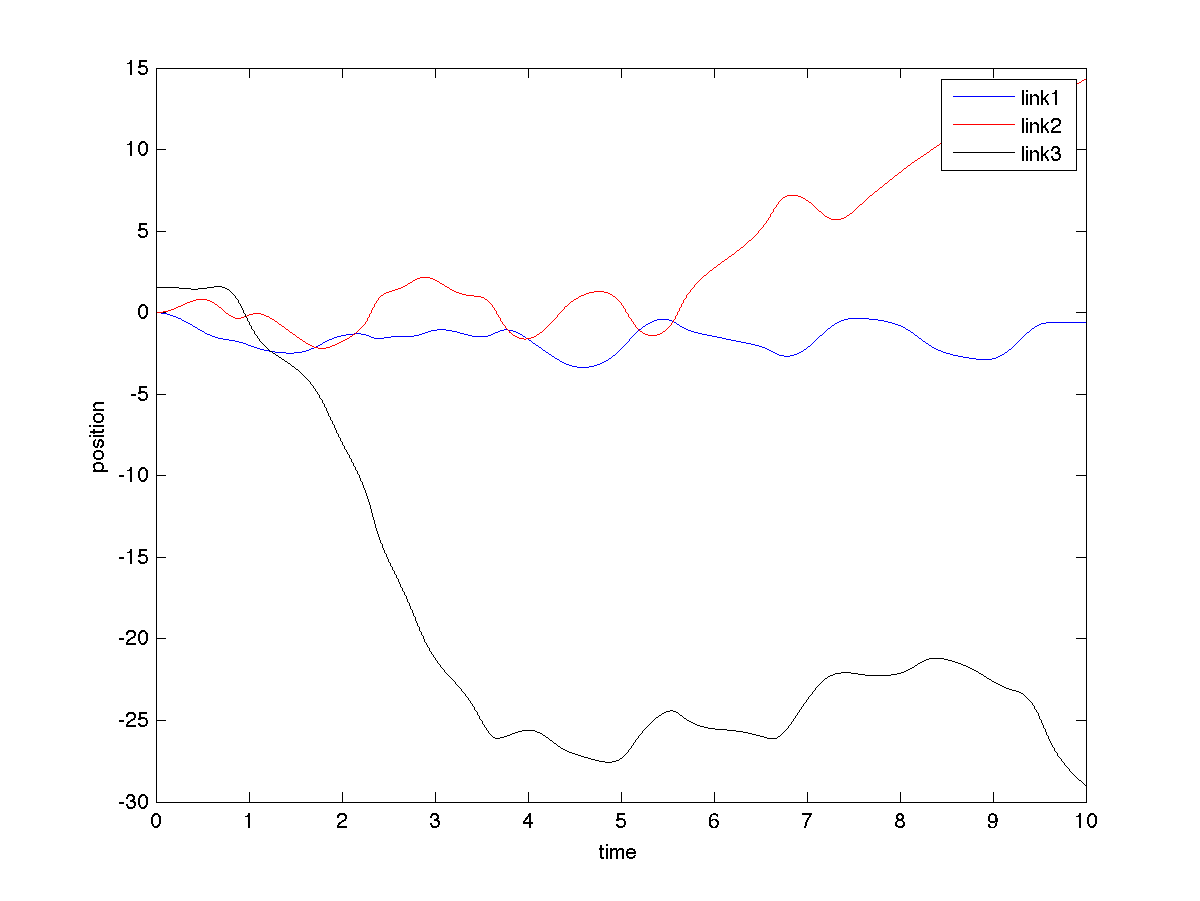
\includegraphics[scale=0.5]{hw10_4.png}
\end{center}

\section{Appendix}
\begin{center}
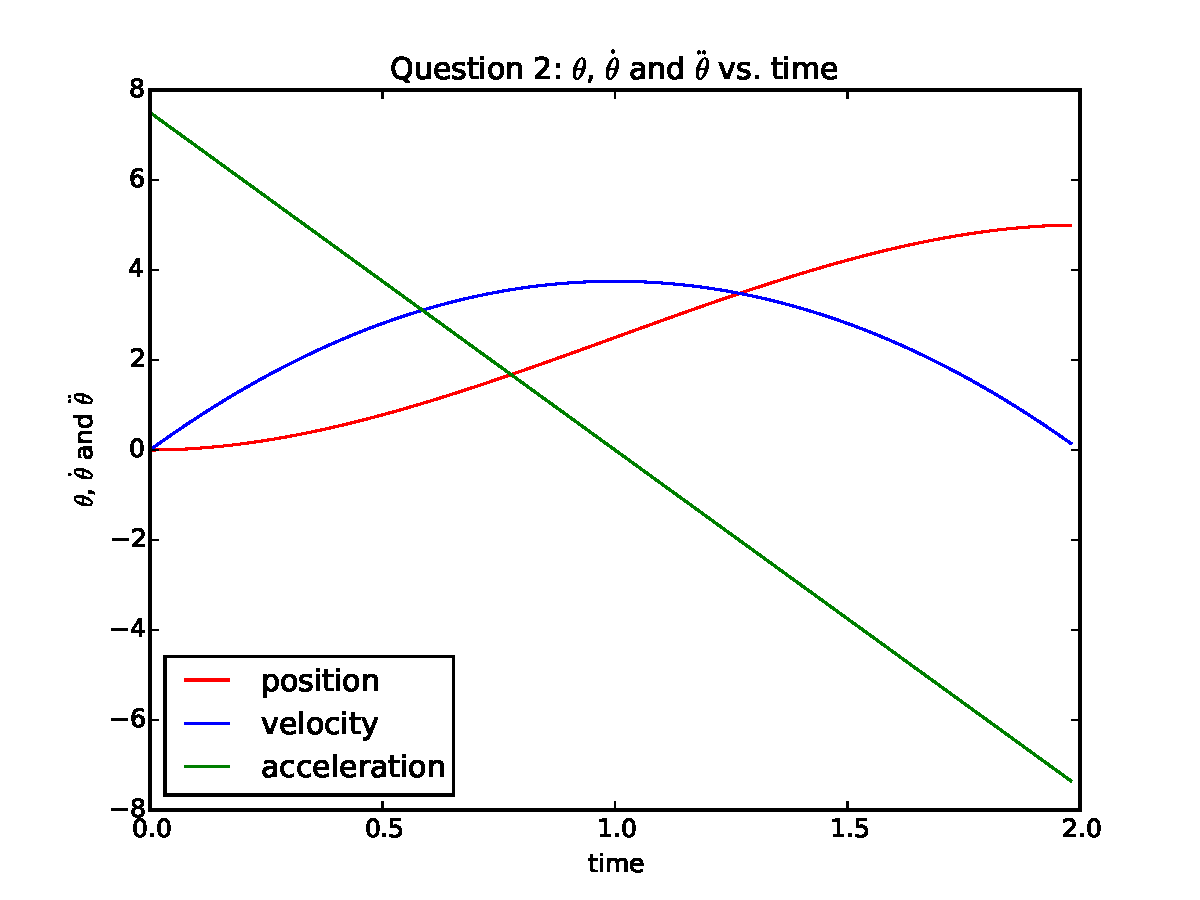
\includegraphics[scale=0.5]{homework10plots.pdf}
\end{center}
\end{document}
